% This file was created with matplot2tikz v0.4.0.
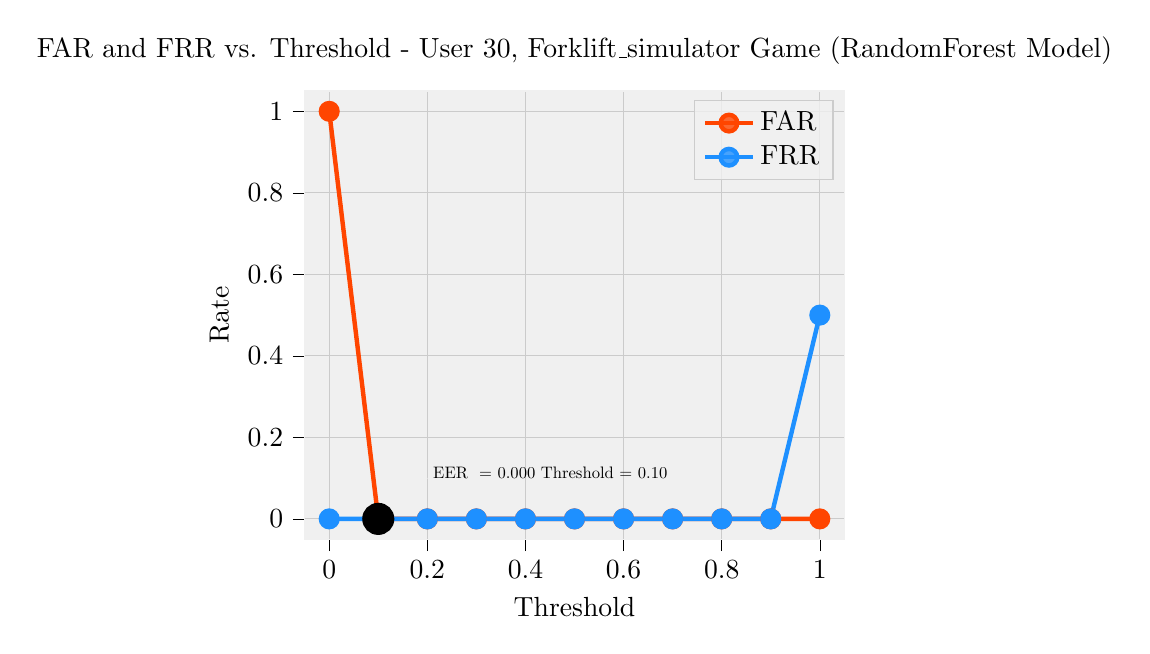
\begin{tikzpicture}

\definecolor{dodgerblue}{RGB}{30,144,255}
\definecolor{lightgray203}{RGB}{203,203,203}
\definecolor{lightgray204}{RGB}{204,204,204}
\definecolor{orangered}{RGB}{255,69,0}
\definecolor{whitesmoke240}{RGB}{240,240,240}

\begin{axis}[
axis background/.style={fill=whitesmoke240},
axis line style={whitesmoke240},
legend cell align={left},
legend style={fill opacity=0.8, draw opacity=1, text opacity=1, draw=lightgray204, fill=whitesmoke240},
tick align=outside,
tick pos=left,
title={FAR and FRR vs. Threshold - User 30, Forklift\_simulator Game (RandomForest Model)},
x grid style={lightgray203},
xlabel={Threshold},
xmajorgrids,
xmin=-0.05, xmax=1.05,
xtick style={color=black},
y grid style={lightgray203},
ylabel={Rate},
ymajorgrids,
ymin=-0.05, ymax=1.05,
ytick style={color=black}
]
\addplot [ultra thick, orangered, mark=*, mark size=3, mark options={solid}]
table {%
0 1
0.1 0
0.2 0
0.3 0
0.4 0
0.5 0
0.6 0
0.7 0
0.8 0
0.9 0
1 0
};
\addlegendentry{FAR}
\addplot [ultra thick, dodgerblue, mark=*, mark size=3, mark options={solid}]
table {%
0 0
0.1 0
0.2 0
0.3 0
0.4 0
0.5 0
0.6 0
0.7 0
0.8 0
0.9 0
1 0.5
};
\addlegendentry{FRR}
\addplot [ultra thick, black, mark=*, mark size=5, mark options={solid}, only marks, forget plot]
table {%
0.1 0
};
\draw[->,draw=whitesmoke240] (axis cs:0.2,0.1) -- (axis cs:0.1,0);
\draw (axis cs:0.2,0.1) node[
  scale=0.6,
  anchor=base west,
  text=black,
  rotate=0.0,
  align=left
]{EER ~= 0.000
Threshold = 0.10};
\end{axis}

\end{tikzpicture}
